\section{RL and the Real World}

% ---------------------------------------------------------------- Slide 46 (divider)
\begin{frame}{}
    \LARGE Reinforcement Learning and the \textbf{Real World}
\end{frame}

% ---------------------------------------------------------------- Slide 47
\begin{frame}{}
\vfill
\begin{columns}[c]
\begin{column}{0.5\textwidth}
\centering
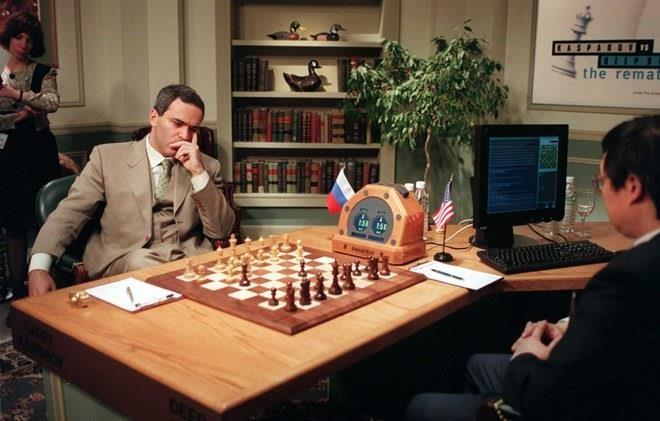
\includegraphics[width=\linewidth]{images/meta-rl-open/figures/deepblue-chess.jpg}
\end{column}
\begin{column}{0.5\textwidth}
\centering
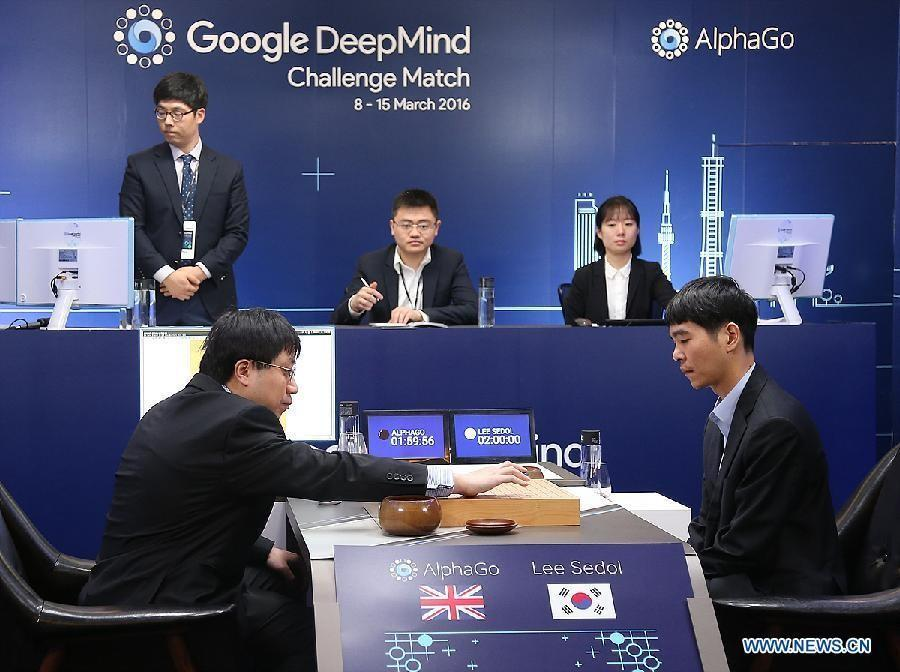
\includegraphics[width=\linewidth]{images/meta-rl-open/figures/alphago-match.jpg}
\end{column}
\end{columns}
\vfill
\end{frame}

% ---------------------------------------------------------------- Slide 48
\begin{frame}{Moravec's paradox}
\begin{columns}[c]
\begin{column}{0.52\textwidth}
\footnotesize
Moravec's paradox seems like a statement about AI but it is actually a statement about
the physical universe.
\vfill
\centering
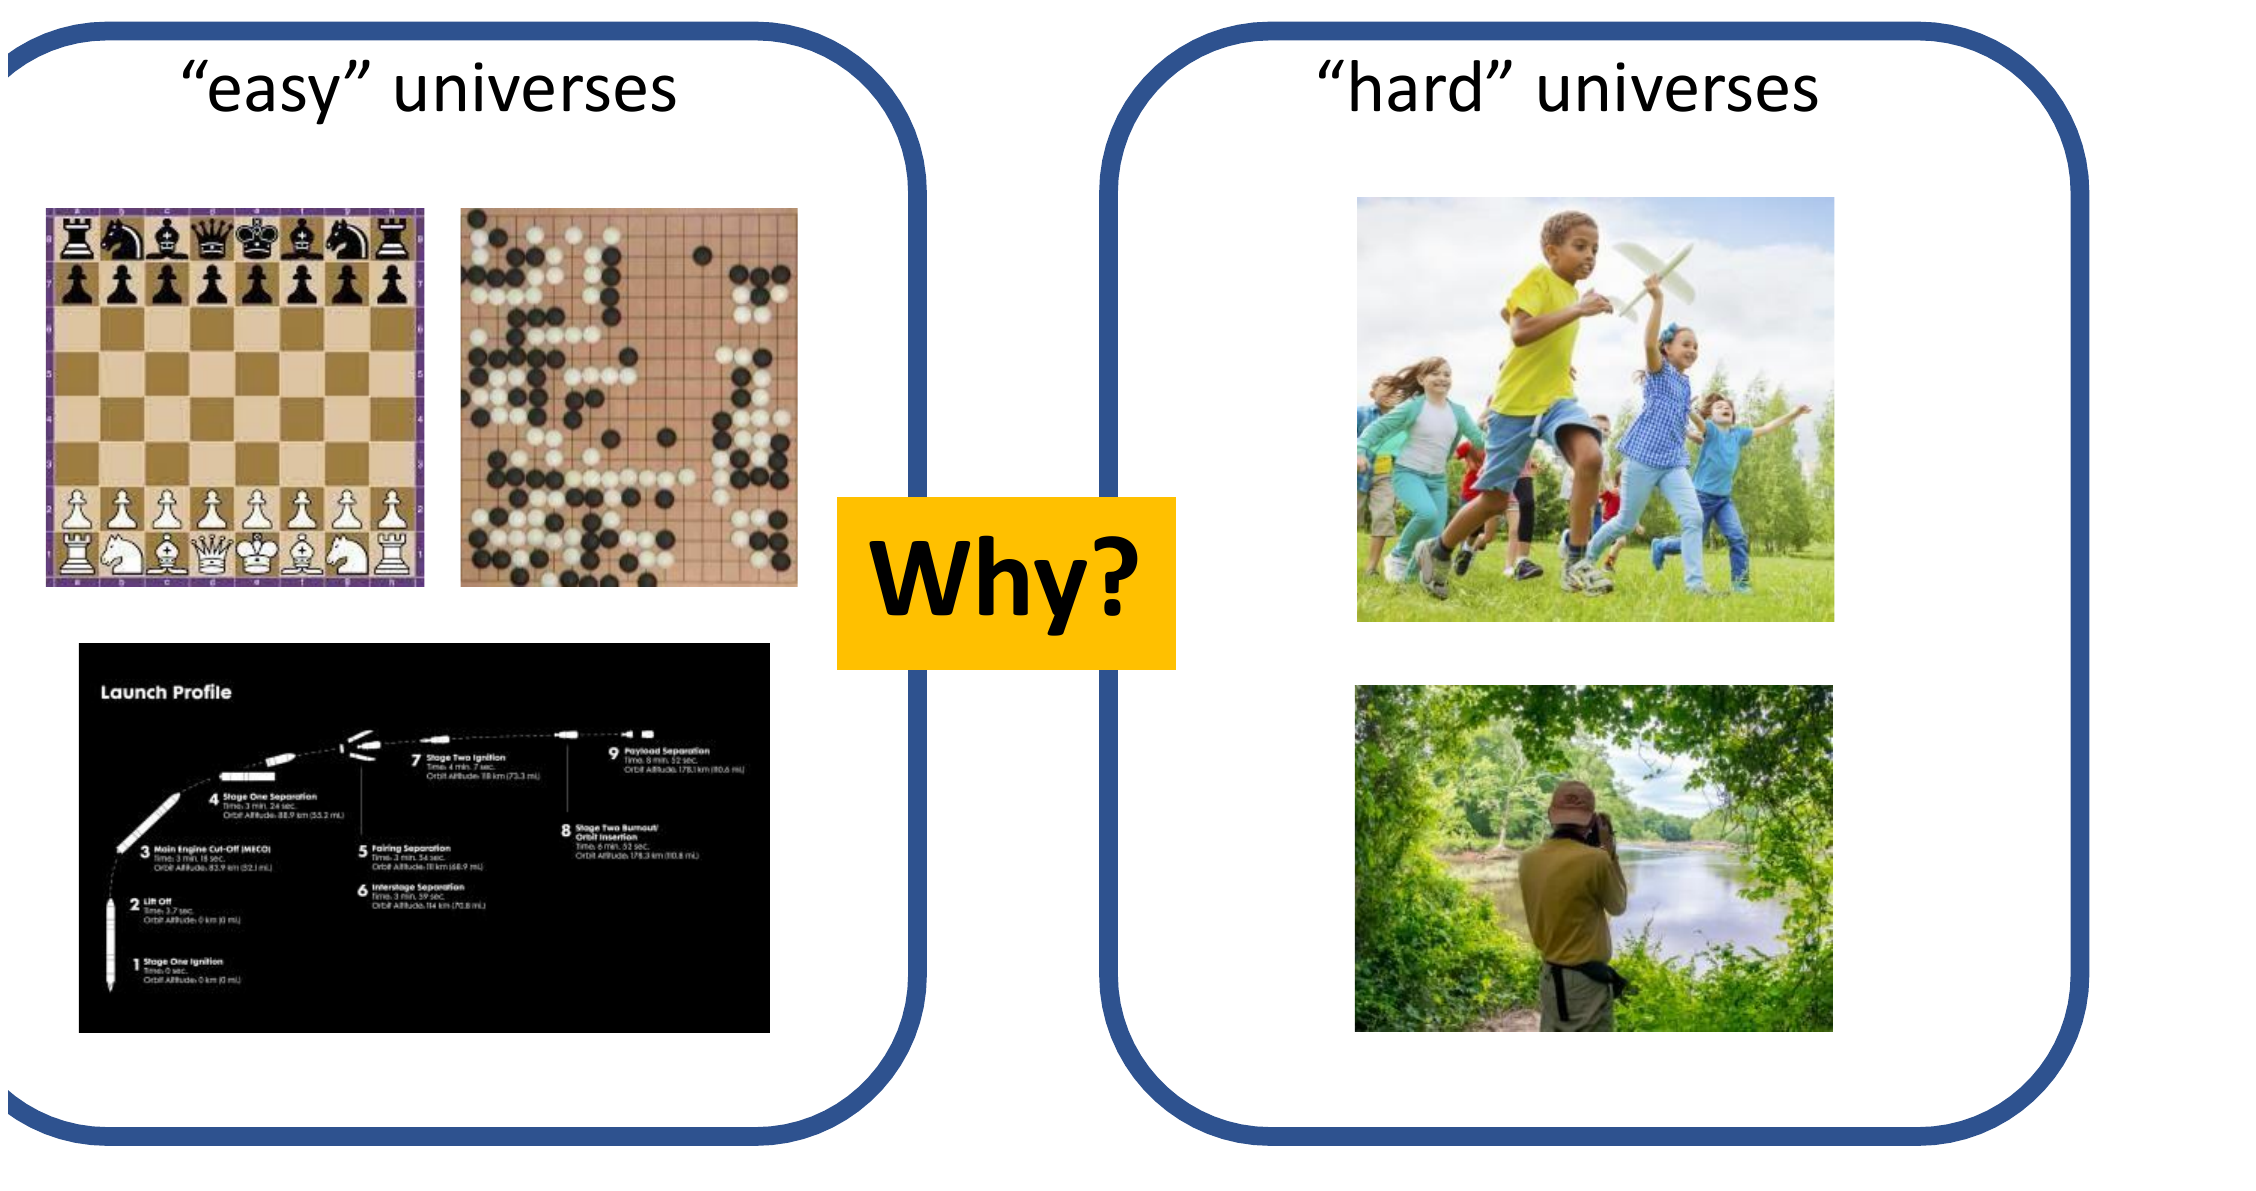
\includegraphics[width=\linewidth]{images/meta-rl-open/figures/moravec-univ.jpg}
\end{column}
\begin{column}{0.48\textwidth}
\tiny
``We are all prodigious olympians in perceptual and motor areas, so good that we make
the difficult look easy. Abstract thought, though, is a new trick, perhaps less than 100
thousand years old. We have not yet mastered it. It is not all that intrinsically
difficult; it just seems so when we do it.'' \hfill -- Hans Moravec
\vspace{0.6em}

``The main lesson of thirty-five years of AI research is that the hard problems are easy
and the easy problems are hard. The mental abilities of a four-year-old that we take for
granted -- recognizing a face, lifting a pencil, walking across a room, answering a
question -- in fact solve some of the hardest engineering problems ever conceived.''
\hfill -- Steven Pinker
\end{column}
\end{columns}
\end{frame}

% ---------------------------------------------------------------- Slide 49
\begin{frame}{What does this have to do with RL?}
\begin{columns}[c]
\begin{column}{0.34\textwidth}
\centering
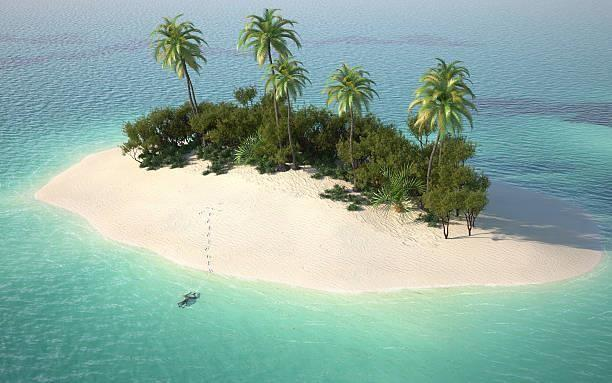
\includegraphics[width=\linewidth]{images/meta-rl-open/figures/island.jpg}
\end{column}
\begin{column}{0.66\textwidth}
\centering How do we engineer a system that can deal with the unexpected?
\vspace{0.6em}
\begin{itemize}
    \item Minimal external supervision about what to do
    \item Unexpected situations that require adaptation
    \item Must discover solutions autonomously
    \item Must ``stay alive'' long enough to discover them!
\end{itemize}
\end{column}
\end{columns}
\vfill
\begin{itemize}
    \item Humans are extremely good at this
    \item Current AI systems are extremely bad at this
    \item RL in principle can do this, and nothing else can
\end{itemize}
\end{frame}

% ---------------------------------------------------------------- Slide 50
\begin{frame}{So what's the problem?}
\begin{center}\footnotesize
RL in principle can do this, and nothing else can --- \emph{but we rarely study this kind
of setting in RL research!}
\end{center}
\vfill
\renewcommand{\arraystretch}{1.25}
\centering\footnotesize
\begin{tabular}{p{0.42\textwidth} p{0.42\textwidth}}
\textbf{``easy'' universes} & \textbf{``hard'' universes}\\
\hline
success $=$ high reward (``optimal control'') & success $=$ ``survival'' (``good enough control'')\\
closed world, rules are known & open world, everything must come from data\\
lots of simulation & no simulation (because rules are unknown)\\
Main question: can RL algorithms optimize really well & Main question: can RL generalize and adapt\\
\end{tabular}
\vfill
{\footnotesize RL should be really good in the ``hard'' universes!}
\end{frame}

% ---------------------------------------------------------------- Slide 51
\begin{frame}{Some questions that come up in the real world}
\begin{columns}[c]
\begin{column}{0.6\textwidth}
\begin{itemize}\footnotesize
    \setlength{\itemsep}{0.5em}
    \item How do we tell RL agents what we want them to do?
    \item How can we learn fully autonomously in continual environments?
    \item How do remain robust as the environment changes around us?
    \item What is the right way to generalize using experience \& prior data?
    \item What is the right way to bootstrap exploration with prior experience?
\end{itemize}
\end{column}
\begin{column}{0.4\textwidth}
\centering
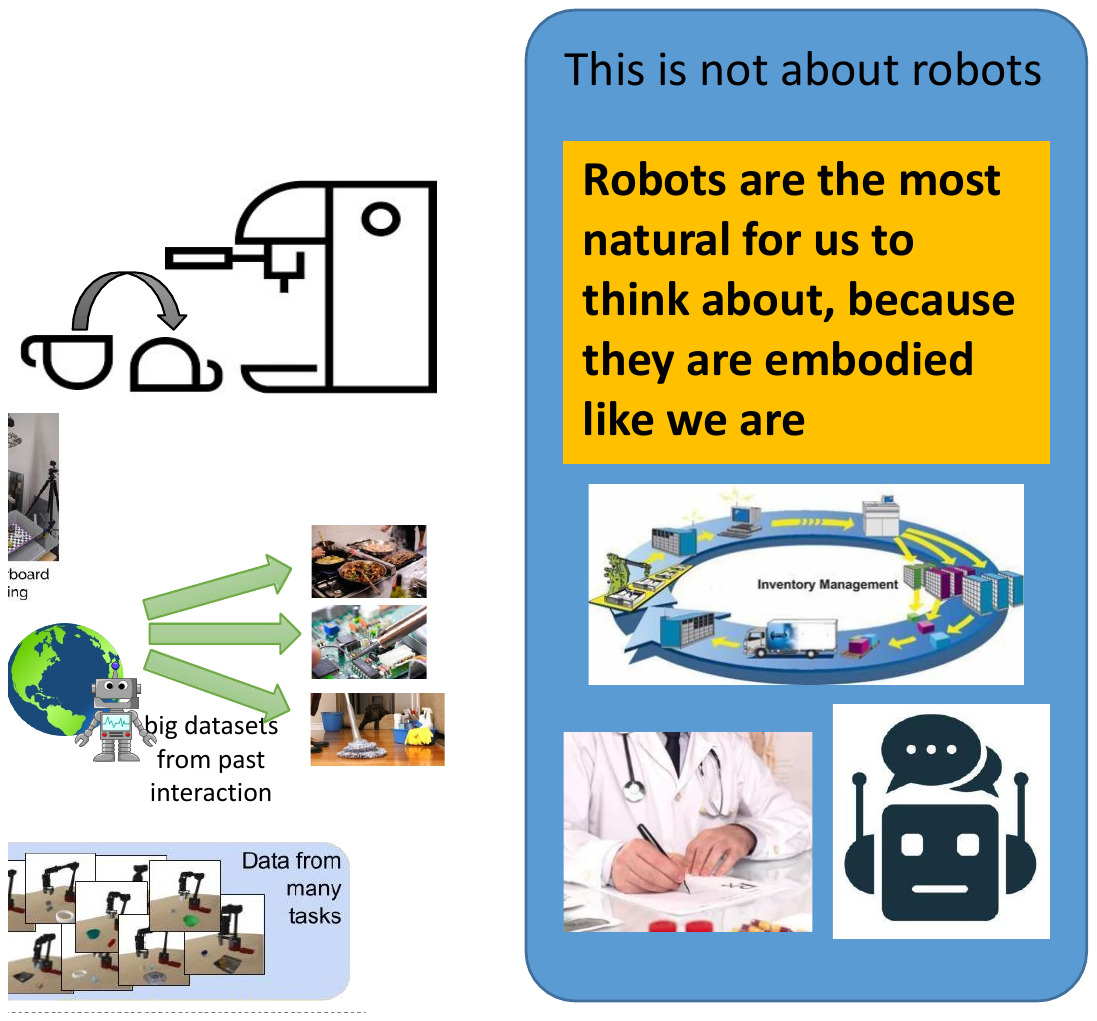
\includegraphics[width=\linewidth]{images/meta-rl-open/figures/realworld-qs.jpg}\\[0.2em]
{\scriptsize This is not about robots --- robots are just the most natural for us to
think about, because they are embodied like we are}
\end{column}
\end{columns}
\end{frame}

% ---------------------------------------------------------------- Slide 52
\begin{frame}{Other ways to communicate objectives?}
\begin{columns}[c]
\begin{column}{0.46\textwidth}
\centering
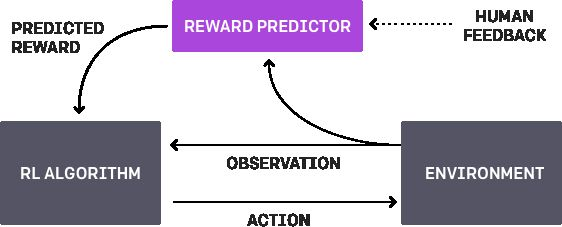
\includegraphics[width=\linewidth]{images/meta-rl-open/figures/christiano-diagram.jpg}\\[0.8em]
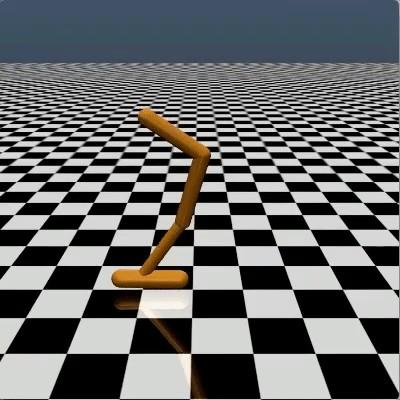
\includegraphics[width=0.6\linewidth]{images/meta-rl-open/figures/christiano-walker.jpg}
\end{column}
\begin{column}{0.54\textwidth}
\centering
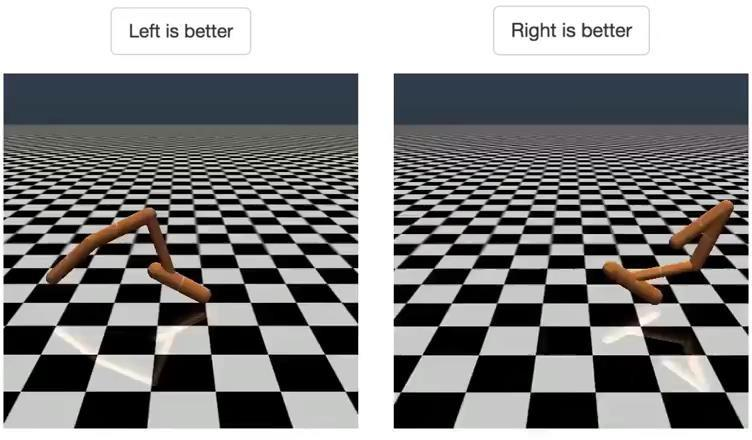
\includegraphics[width=\linewidth]{images/meta-rl-open/figures/christiano-compare.jpg}
\end{column}
\end{columns}
\vfill
{\scriptsize Christiano, Leike, Brown, Martic, Legg, Amodei. \href{https://arxiv.org/abs/1706.03741}{Deep reinforcement learning from human preferences}. 2017.}
\end{frame}

% ---------------------------------------------------------------- Slide 53
\begin{frame}{How can we learn fully autonomously?}
\centering
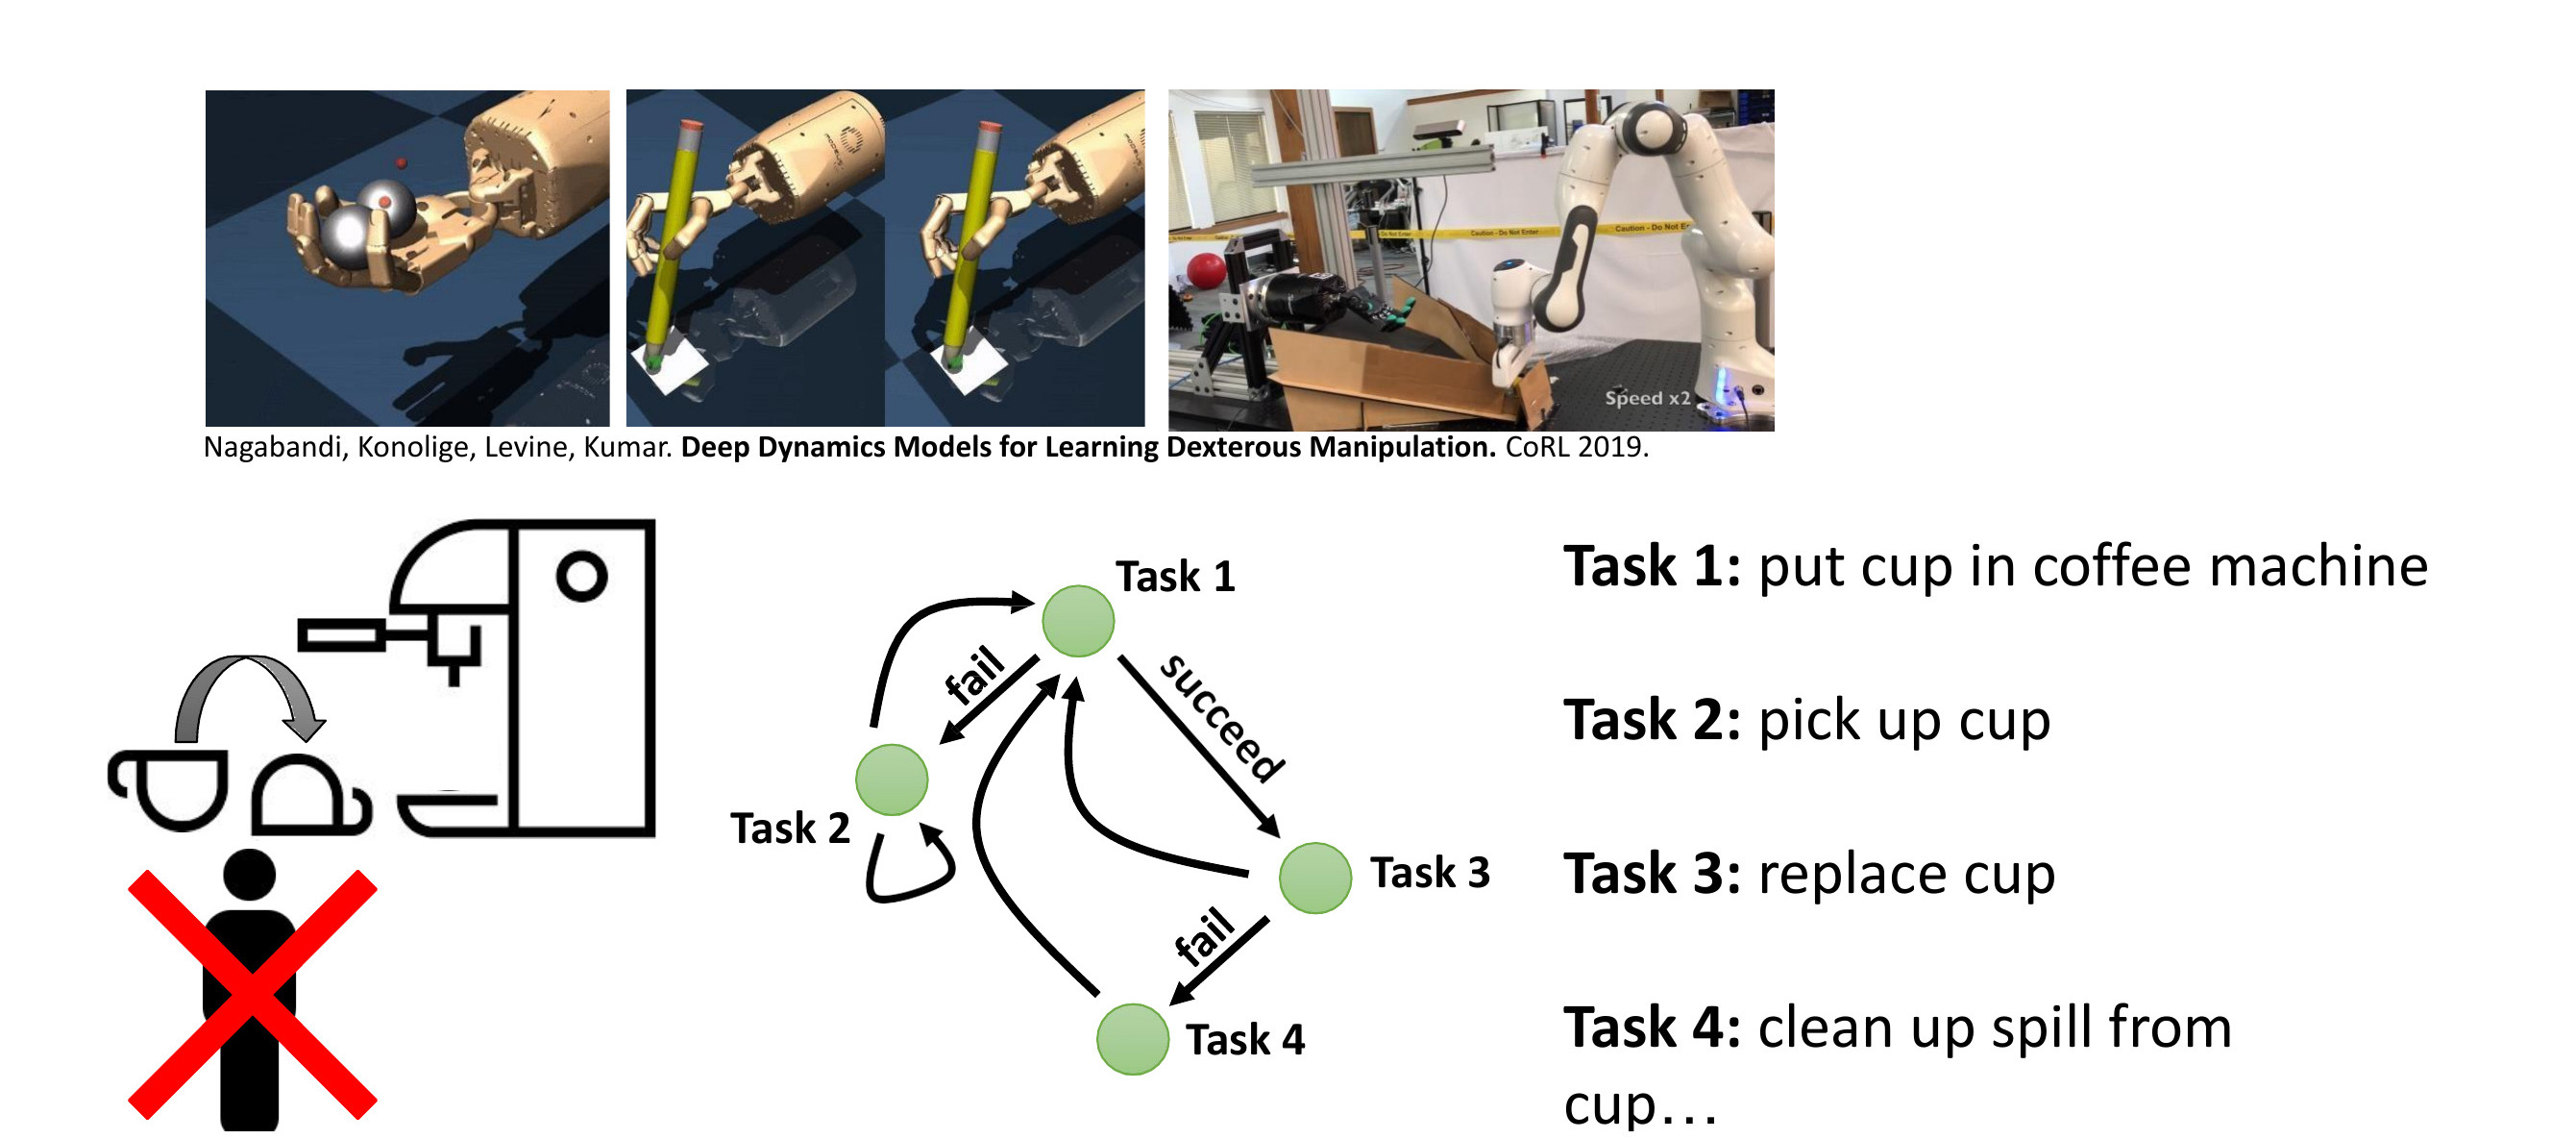
\includegraphics[width=\linewidth,height=0.78\textheight,keepaspectratio]{images/meta-rl-open/figures/nagabandi-tasks.jpg}

\vspace{0.3em}
{\scriptsize Nagabandi, Konolige, Levine, Kumar. Deep Dynamics Models for Learning Dexterous Manipulation. CoRL 2019.}
\end{frame}

% ---------------------------------------------------------------- Slide 54
\begin{frame}{How can we learn fully autonomously?}
\centering
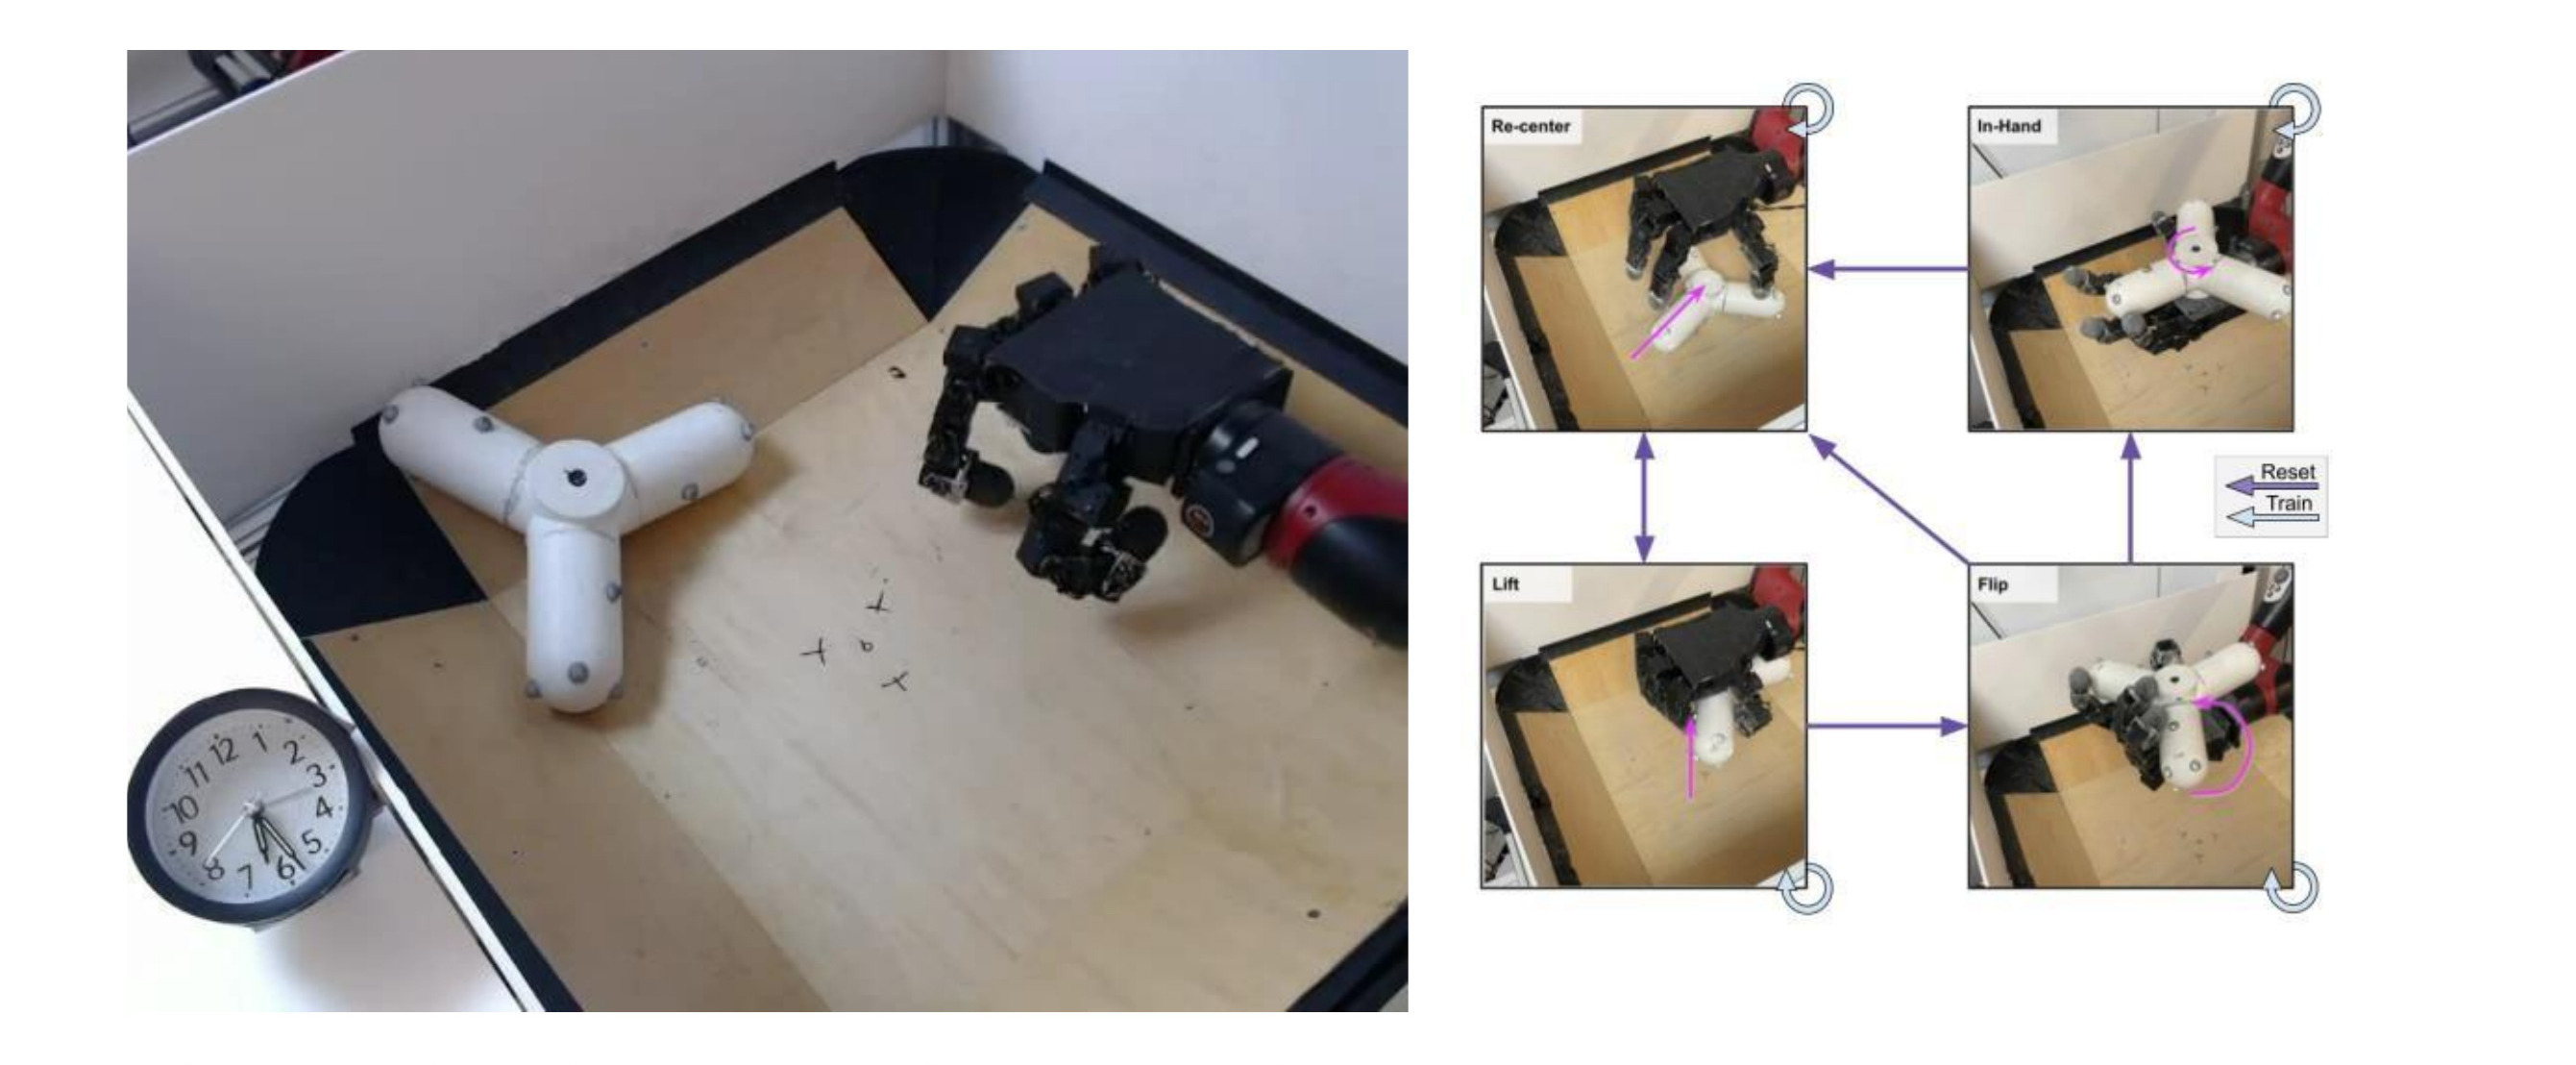
\includegraphics[width=\linewidth,height=0.78\textheight,keepaspectratio]{images/meta-rl-open/figures/reset-free.jpg}

\vspace{0.3em}
{\scriptsize Gupta, Yu, Zhao, Kumar, Rovinsky, Xu, Devlin, Levine. Reset-Free Reinforcement Learning via Multi-Task Learning. 2021.}
\end{frame}

% ---------------------------------------------------------------- Slide 55
\begin{frame}{How to bootstrap exploration from experience?}
\centering
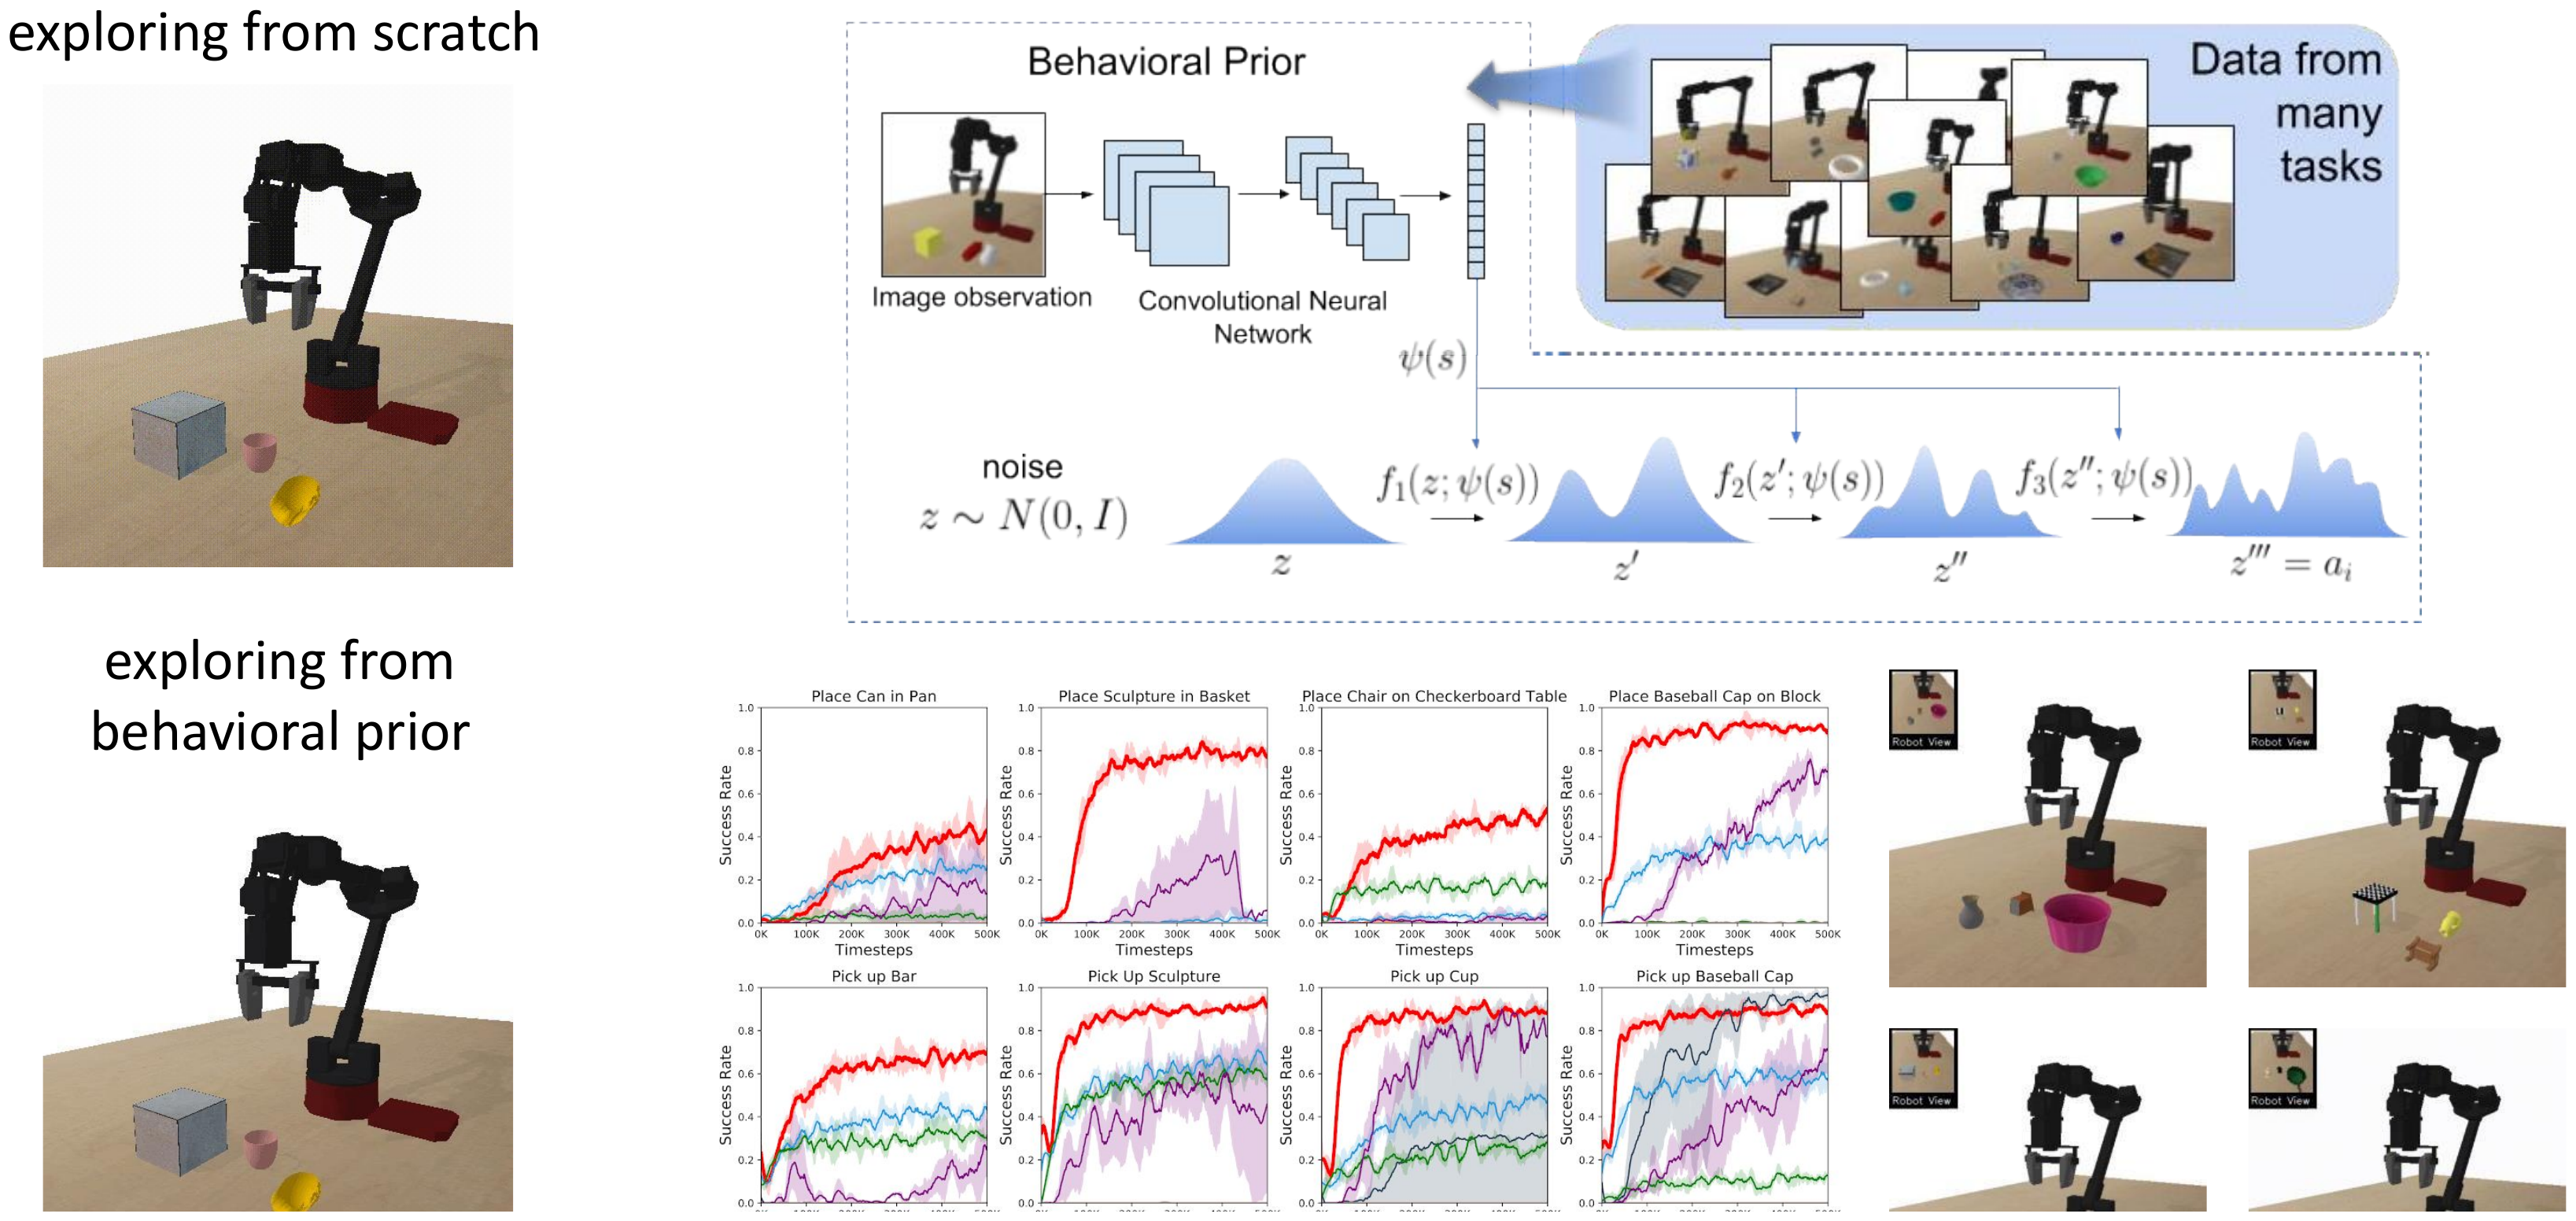
\includegraphics[width=\linewidth,height=0.80\textheight,keepaspectratio]{images/meta-rl-open/figures/parrot-full.png}

\vspace{0.3em}
{\scriptsize Singh*, Hui*, Zhou, Yu, Rhinehart, Levine. Parrot: Data-driven behavioral priors for reinforcement learning. 2020.}
\end{frame}

% ---------------------------------------------------------------- Slide 56
\begin{frame}{This all seems really hard, what's the point?}
\begin{columns}[c]
\begin{column}{0.32\textwidth}
\centering
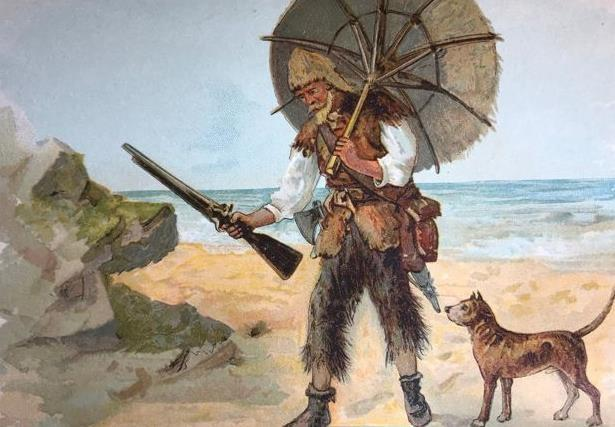
\includegraphics[width=\linewidth]{images/meta-rl-open/figures/crusoe.jpg}
\end{column}
\begin{column}{0.68\textwidth}
\begin{center}Why is this interesting?\end{center}
\vspace{0.3em}
\begin{itemize}
    \item It's exciting to see what solutions intelligent agents come up with
    \item Most exciting if they come up with something we don't expect
    \item This requires the world they inhabit to admit novel solutions
    \item This means that world must be complicated enough!
\end{itemize}
\end{column}
\end{columns}
\vfill
{\footnotesize To see interesting emergent behavior, we must train our systems in
environments that actually require interesting emergent behavior!}

{\footnotesize RL in the real world may be difficult, but it is also rewarding.}
\end{frame}
